%Łukasz DZIEŁ
%tel: +48 883 533 374
%email: lukasz.dziel@wat.edu.pl
%wersja: 20220316
%testowano w środowisku: TeXLive2021 (instalacja pełna z iso) + TeXstudio 4.2.2

%Łukasz DZIEŁ
%tel: +48 883 533 374
%email: lukasz.dziel@wat.edu.pl
%wersja: 20220316
%testowano w środowisku: TeXLive2021 (instalacja pełna z iso) + TeXstudio 4.2.2

\documentclass[13pt, a4paper, twoside]{scrartcl}

\usepackage[left=20mm,right=20mm,top=25mm,bottom=25mm,bindingoffset=10mm]{geometry}
\usepackage[T1]{fontenc}
\usepackage[polish]{babel}
\usepackage[utf8]{inputenc}

\usepackage{mathptmx}
\usepackage{courier}

\usepackage[normalem]{ulem}

\usepackage{sectsty}
\allsectionsfont{\normalfont\bfseries\fontsize{14}{18}\selectfont}

\usepackage[titles]{tocloft}
\setcounter{tocdepth}{2}
\renewcommand{\cftsecfont}{\fontsize{12}{14}\selectfont}
\renewcommand{\cftsecpagefont}{\fontsize{12}{14}\selectfont}
\renewcommand{\cftsecleader}{\fontsize{12}{14}\selectfont\cftdotfill{1}}
\renewcommand{\cftsecindent}{0mm}
\renewcommand{\cftsecnumwidth}{22mm}
\renewcommand{\cftsecaftersnum}{. }
\renewcommand{\cftbeforesecskip}{2mm}

\renewcommand{\cftsubsecfont}{\fontsize{11}{13}\selectfont}
\renewcommand{\cftsubsecpagefont}{\fontsize{11}{13}\selectfont}
\renewcommand{\cftsubsecindent}{5mm}
\renewcommand{\cftsubsecnumwidth}{8mm}
\renewcommand{\cftsubsecaftersnum}{. }
\renewcommand{\cftbeforesubsecskip}{2mm}
\renewcommand{\cftsubsecleader}{\fontsize{11}{13}\selectfont\cftdotfill{1}}

\renewcommand{\cftsubsubsecfont}{\fontsize{11}{13}\selectfont}
\renewcommand{\cftsubsubsecpagefont}{\fontsize{11}{13}\selectfont}
\renewcommand{\cftsubsubsecindent}{5mm}
\renewcommand{\cftsubsubsecnumwidth}{12mm}
\renewcommand{\cftsubsubsecaftersnum}{. }
\renewcommand{\cftbeforesubsubsecskip}{0mm}
\renewcommand{\cftsubsubsecleader}{\fontsize{11}{13}\selectfont\cftdotfill{1}}

\renewcommand{\cftfigindent}{0mm}
\renewcommand{\cftfignumwidth}{15mm}
\renewcommand{\cftfigpresnum}{Rys. }
\renewcommand{\cftfigaftersnum}{. }
\renewcommand{\cftfigleader}{\normalfont\cftdotfill{1}}

\renewcommand{\cfttabindent}{0mm}
\renewcommand{\cfttabnumwidth}{15mm}
\renewcommand{\cfttabpresnum}{Tab. }
\renewcommand{\cfttabaftersnum}{. }
\renewcommand{\cfttabfont}{\normalfont}
\renewcommand{\cfttableader}{\normalfont\cftdotfill{1}}

\usepackage{amsmath,amsfonts,amsthm}

\usepackage{color}
\usepackage{float}

\usepackage{verbatimbox}
\def\verbarg{{\fontsize{11}{13}\selectfont\makebox[7mm]{\arabic{VerbboxLineNo}}}\hspace{12mm}}

\usepackage[plain]{algorithm}
\floatstyle{plaintop}
\restylefloat{algorithm}
\floatname{algorithm}{Alg.}

\usepackage[pdftex]{graphicx}

\renewcommand\thesection{Rozdział \Roman{section}}
\renewcommand\thesubsection{\Roman{section}.\arabic{subsection}}
% \renewcommand\thesubsubsection{\Roman{section}.\arabic{subsection}.\arabic{subsubsection}}

\usepackage{longtable}
\usepackage[font=bf, labelfont=bf, belowskip=-0mm]{caption}
\captionsetup[figure]{name=Rys., labelsep=period}
\captionsetup[table]{name=Tab.,  labelsep=period}
\captionsetup[lstlisting]{margin=0pt, font=bf, labelsep=period}
\captionsetup[algorithm]{font=bf, labelsep=period}

\usepackage{listings}
\usepackage{color}

\usepackage{xurl}
\urlstyle{ttfamily}


\newcommand{\myparagraph}[1]{\paragraph{#1}\mbox{}\\}
\newcommand{\myurl}[1]{\urlstyle{same}\url{#1}}

\usepackage{hyperref}
\usepackage{pdfpages}


\usepackage{fancyhdr}
\pagestyle{fancy}
\fancyhead[RO, LE]{\thepage}
\fancyhead[RE, LO]{}
\fancyfoot{}
\renewcommand\headrulewidth{0pt}

\fancypagestyle{firststyle}{
\fancyhead[RO, LE]{}
\fancyhead[RE, LO]{}
}

\setlength\parindent{27pt}

\newcommand{\inserttitlepage}{
    \thispagestyle{firststyle}
    \begin{center}
        \fontsize{22}{14}\textbf{WOJSKOWA~~AKADEMIA~~TECHNICZNA}\\
        \fontsize{12}{10}\textbf{im. Jarosława Dąbrowskiego}
    \end{center}
    \vspace{-7mm}
    \rule{\linewidth}{0.5pt}
    \begin{center}
        \fontsize{20}{10}{\textbf{WYDZIAŁ~~CYBERNETYKI}}
    \end{center}
    
    \vspace{5mm}
    
    \begin{center}
        
\includegraphics[width=40mm]{./defs/WAT.png}
    \end{center}

    \vspace{0mm}

    \begin{center}
        {{\fontsize{26}{10} \selectfont {PRACA DYPLOMOWA}}}\\
        \vspace{3mm}
        {\fontsize{20}{10} \selectfont \stopien}
    \end{center}
    
    \vspace{5mm}
    
    \begin{longtable*}{p{.18\textwidth} p{.75\textwidth}}
        \fontsize{14}{20}\selectfont{Temat pracy:} &\fontsize{16}{20}\selectfont{\textbf{\noindent\temat}} \\
    \end{longtable*}
    
    \vspace{5mm}
    
    \begin{center}
        \textrm{\textbf{\fontsize{14}{20}\selectfont{\kierunek}}}\\
        \scriptsize\textrm{...........................................................................................................\\{{\scriptsize{(kierunek studiów)}}}}\\~\\
        \vspace{5mm}    
        \textrm{\textbf{\fontsize{14}{20}\selectfont{\specjalnosc}}}\\
        \scriptsize\textrm{...........................................................................................................\\\scriptsize{(specjalność)}}\\
    \end{center}
   
    \vspace{5mm}

    \begin{longtable*}{p{.509\textwidth} p{.5\textwidth}}
        \textrm{Dyplomant:}\vspace{5mm} & 	\textrm{Promotor:}\\
        \textrm{\textbf{\autor}}  & \textrm{\textbf{\promotor}} \\
    \end{longtable*}
    
    \begin{center} 
    \rule{\linewidth}{0.5pt}
    \fontsize{12}{10} \textbf{\data} \end{center}
    
     
    \clearpage
    

    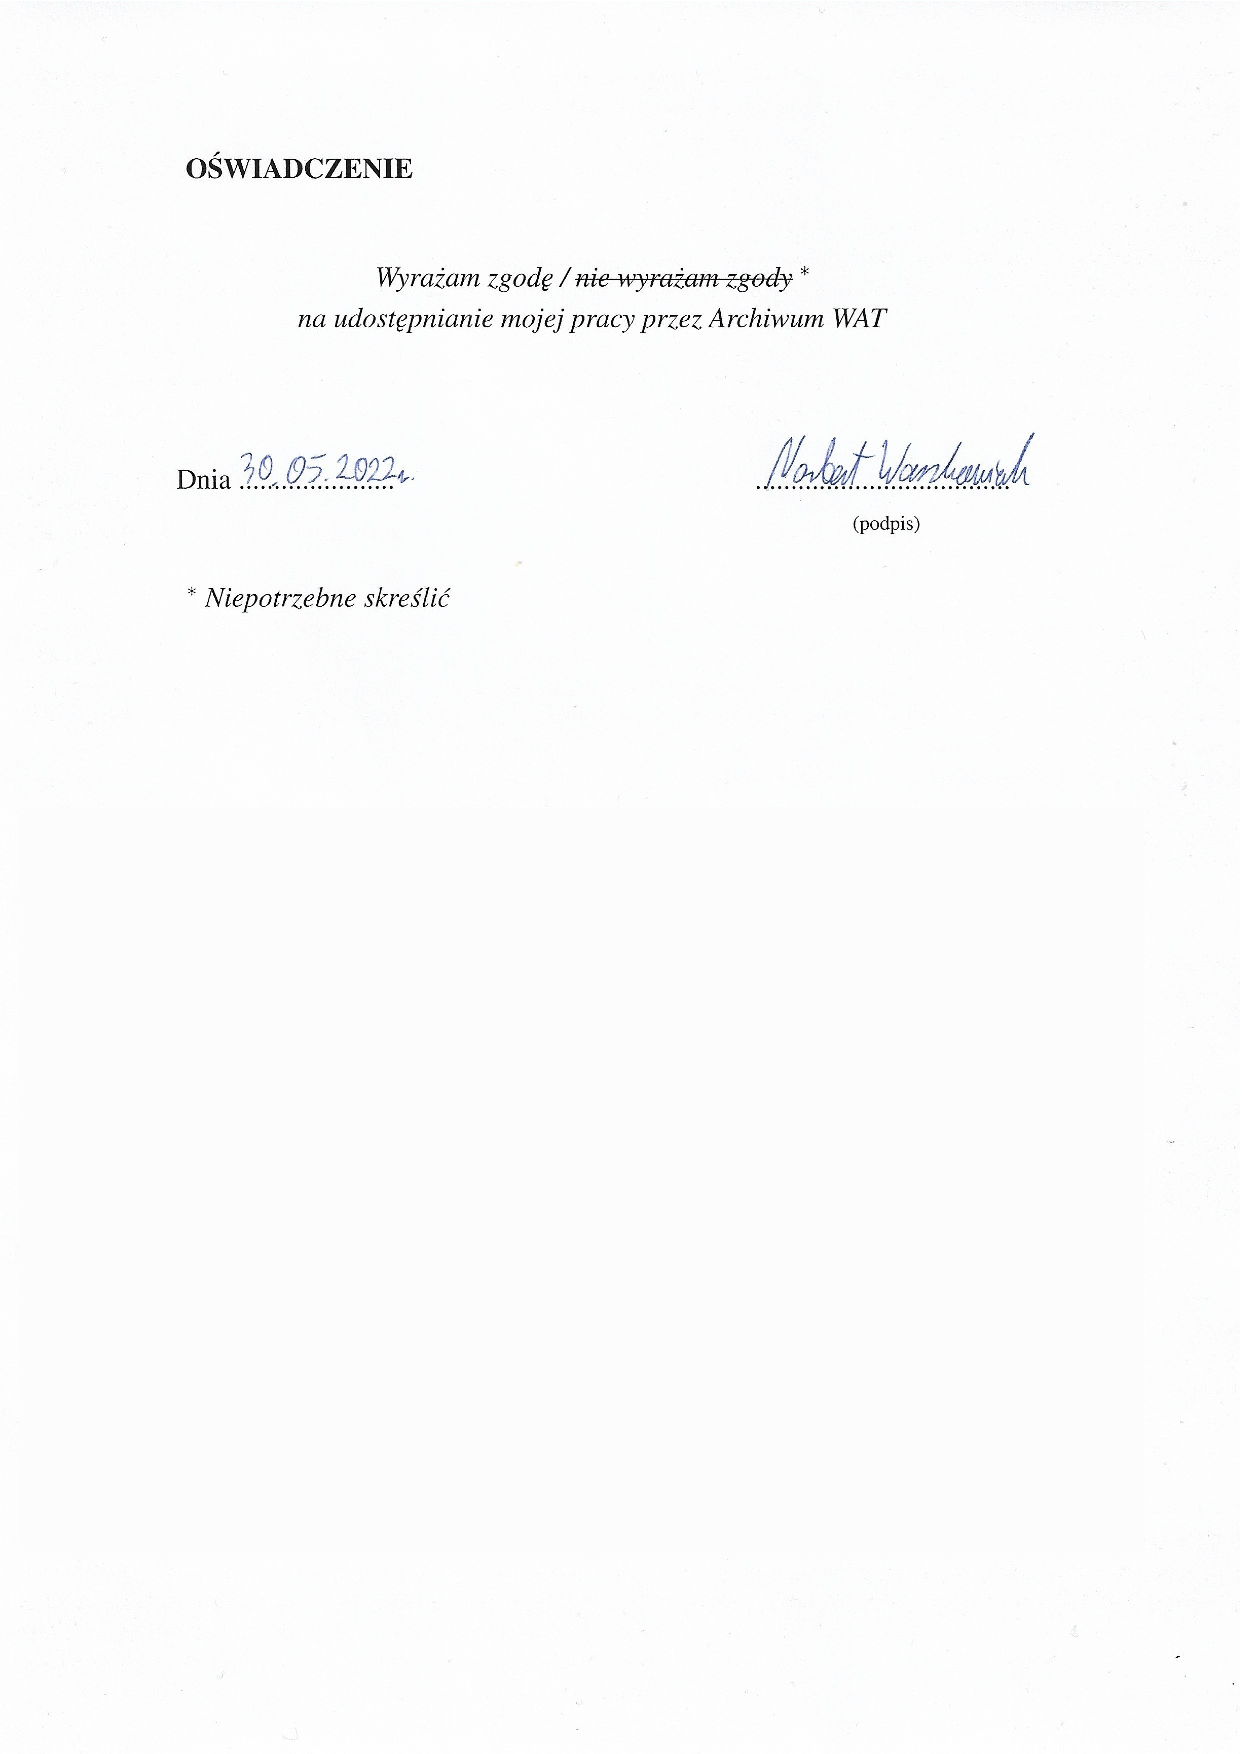
\includepdf[pages=-]{oswiadczenie.pdf}  

    \normalsize
    
    \tableofcontents
    
    \newpage
}

\defcaptionname{polish}{\refname}{Bibliografia}

\definecolor{mygray}{rgb}{0.95,0.95,0.95}

\renewcommand{\lstlistingname}{Kod.}

\lstset{
    basicstyle=\ttfamily\scriptsize,
    numbers=left,
    numberstyle=\ttfamily\scriptsize\color{black},
    numbersep=10pt,
    showspaces=false,
    breaklines=true,
    keepspaces=true,
    tabsize=2,
    xleftmargin=10pt,
    framexleftmargin=5pt,
    captionpos=tc,
    backgroundcolor=\color{mygray},
    keywordstyle=\color{black},
    inputencoding=utf8
}

\newcommand{\source}[1]{\vspace{0mm} \noindent\fontsize{10}{10}\selectfont{Źródło: {#1}}\normalsize\vspace{0mm}}

\newcommand{\TODO}[1]{
    {\large \color{red}{\underline{\textbf{TODO: #1}}}} 
}
\newcommand{\kierunek}{INFORMATYKA}
\newcommand{\stopien}{STUDIA II$^{\mathrm{o}}$} %Odpowiednie usunąć
\newcommand{\temat}{MOBILNY SYSTEM ZARZĄDZANIA I STEROWANIA BEZPILOTOWYM STATKIEM LATAJĄCYM}
\newcommand{\data}{Warszawa 2022}
\newcommand{\autor}{Norbert WASZKOWIAK}
\newcommand{\promotor}{dr inż. Michał DYK}
\newcommand{\zgoda}{TAK} %W przypadku braku zgody zakomentować tą linię
\newcommand{\specjalnosc}{SYSTEMY INFORMATYCZNE}
\newcommand{\bibTitle}[1]{``#1''}



\begin{document}

\inserttitlepage

\section*{Wstęp} 
\addcontentsline{toc}{section}{Wstęp}
    
% Zwarte wprowadzenie w temat i cele pracy z nawiązaniem do dziedziny przedmiotowej oraz rozwiązanego problemu. Uzasadnienie potrzeby i zastosowania wyników pracy. Przedstawienie układu i streszczenie zawartości rozdziałów pracy (2-3 zdania na rozdział).\\
% Zaleca się, aby tekst wstępu nie przekraczał dwóch stron.
     o skrotach bsp
\clearpage

\section{Prezentacja zagadnienia bezpilotowych statków latających oraz koncepcji ich wykorzystania}
\hspace{1cm}TODO text

\subsection{Definicja BSP}
\hspace{1cm}W nomenklaturze związanej z domeną bezpilotowych statków latających można znaleźć wiele tożsamych terminów na określanie bezpilotowych statków latających, są to m.in.:
\begin{itemize}
  \item Bezzałogowy statek powietrzny, BSP (ang. \textit{unmanned aerial vehicle}, UAV);
  \item Bezzałogowy system powietrzny (ang. \textit{unmanned aerial system}, UAS);
  \item Samolot zdalnie sterowany (ang. \textit{remotely piloted aircraft}, RPA);
  \item Dron (ang. \textit{drone}),
\end{itemize}

Każdy z tych terminów kładzie nacisk na inną cechę, ale wszystkie nadal odnoszą się do jednego obiektu i będą w tej pracy używane zamiennie. Amerykański pisarz zajmujący się zagadnieniami systemów bezzałogowych i technologi obronnych,  Kelsey Artheon na łamach czasopisma "Popular Science" definiuje to pojęcie następująco: "dron oznacza każdy bezzałogowy zdalnie sterowany pojazd latający, bez względu na to, czy jest to malutki, sterowany radiem helikopter-zabawka, czy też ważący 14,5 tony Global Hawk, wart 104 mln dolarów. Jeżeli coś lata i jest sterowane przez pilota z ziemi, to pasuje do potocznej definicji drona". \footnote{A. Kelsey, \textit{Flying Robots 101: Everthing You Need to Know about Drones}, Popular Science\cite{arton-kelsey}} \cite{dron-ibuk} 

\hspace{1cm}Warunkiem koniecznym według autora do zakwalifikowania wehikułu jako bezzałogowy statek powietrzny są:
\begin{itemize}
  \item \textbf{bezpilotowość} - wehikuł na swoim pokładzie nie posiada pilota;
  \item \textbf{dwukierunkowość} - wehikuł musi mieć możliwość powrotu/wylądowania. Jest to podstawowa cecha odróżniająca drony od pocisków manewrujących; 
  \item  \textbf{sterowalność} - możliwość zmiany kierunku lotu w trakcie jego wykonywania.
\end{itemize}

\subsection{Historia BSP}
\hspace{1cm}Bezpilotowe statki latające z racji, że są całkiem nową domeną, mają też stosunkowo krótką, ale interesującą historię.

\subsubsection{Błędnie klasyfikowane wehikuły}
\hspace{1cm}Po zdefiniowaniu czym jest dron, można się zastanowić, co było pierwszym elementem spełniającym tę definicję. Autor tej pracy uważa, że kluczowym elementem umożliwiającym zakwalifikowanie obiektu jako dron jest możliwość zmiany trajektorii lotu w trakcie jego działania. W literaturze często wskazywane są dwa obiekty jako prekursory dronów, tzn. gołąb Archytasa z Tarentu i balony zawierające ładunki wybuchowe wykorzystane w konflikcie między Austrią i Wenecją w 1849 r. Pierwszy rzekomy prekursor nie umożliwia sterowania obiektem po jego wystartowaniu, więc tym samym nie jest to zgodne z przytoczonymi definicjami. Ten wynalazek można uznać za pierwszą rakiet, robota, ale nie drona. Drugi przykład, balony na gorące powietrze również nie mogą zostać uznane za bezzałogowy statek powietrzny z tego samego powody. W dodatku pomysł Austriaków zakończył się niepowodzeniem, ponieważ wiatr zwiał balony na ich własne pozycje.\cite{dron-ibuk}. 


\begin{figure}[!ht]
  \centering
  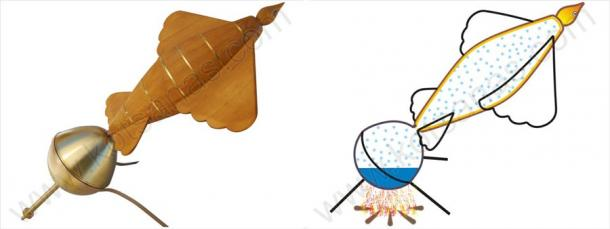
\includegraphics[width=8cm]{./Obrazy/golab.jpg}
  \caption{Latający gołąb Archytasa z Tarentu}
  \source{\myurl{https://input.niezalezna.pl//259fef5fd.jpg}}
  \end{figure}

\subsubsection{Pierwszy pełnoprawny dron}

\hspace{1cm}Podczas I wojny światowej podjęto liczne próby skonstruowania bezpilotowych statków latających, ale żaden z nich nie został ukończony na przed skończeniem wojny. Przykładowo wehikuł Kettering Bug, był w stanie dolecieć na odpowiednią odległość, ale jego sterowanie polegało na wyliczeniu przez operatora dokładną liczbę obrotów silnika, lecz w takim wypadku bliżej takiemu samolotowi bliżej do torpedy niż do drona. 

W 1931r. Królewskie Siły Powietrzne (ang. Royal Air Force) na podstawie samolotu szkolnego \textit{De Havilland DH-60T ”Tiger Moth”} opracowły pierwszy bezpilotowy statek powietrzny \textit{DH-82B "Queen Bee"}. Samolot ten miał służyć jako ruchomy cel do ćwiczeń dla obslugi dział przeciw lotniczych, sterowany przez pilota za pomocą fal radiowych. Jego oficjalna prezentacja została jednak przerwana, ponieważ ówczesne systemy obrony powietrznej były mało skuteczne, do tego stopnia, że strzelającym skończyła się amunicja, zanim zestrzelili oni bezpilotowy samolot. Wehikuł też spełnia wszystkie wymagania określone wcześniej przez autora, więc uznaje on go za pierwszego drona.\cite{queen-bee}\cite{dron-ibuk}

\begin{figure}[!ht]
  \centering
  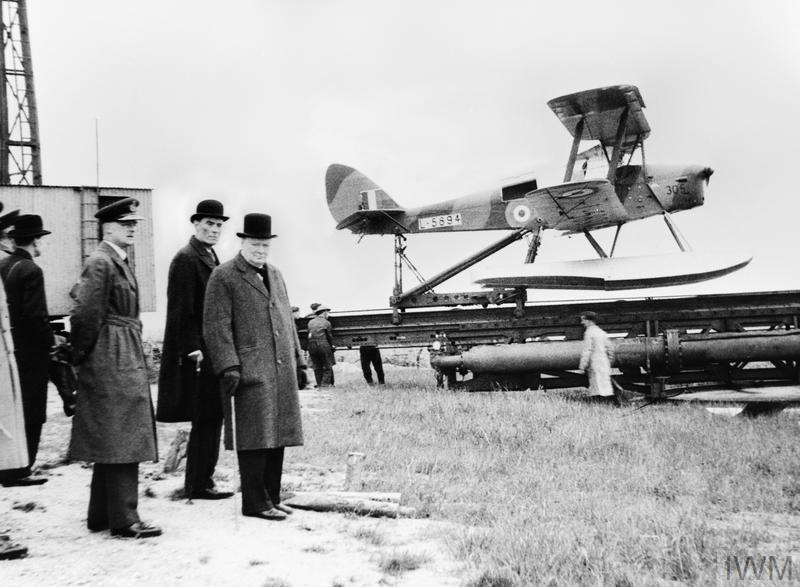
\includegraphics[width=8cm]{./Obrazy/queen-bee.jpg}
  \caption{De Havilland Queen Bee i premier Wielkiej Brytanii Winston Churchill}
  \source{\myurl{https://www.iwm.org.uk/collections/item/object/205195356}}
  \end{figure}

Równolegle w tym samym okresie, a konkretnie w 1935 roku powstał identyczny samolot dla amerykańskich odbiorców: \textit{Radioplane OQ-2}, który był już pierwotnie stworzony jako bezzałogowiec, a nie przez modyfikacje tak jak dron brytyjski.

\subsubsection{Pierwsze drony rozpoznawcze}
\hspace{1cm}W okresie po II wojnie światowej USA kontynuowało prace nad dronami, za pomocą firmy \textit{Ryan Aeronautical Company} i ich serii dronów produkowanych od 1951r. \textit{Firebee}, czego efektem był m.in. \textit{Ryan Model 147 Lightning Bug} opracowany w 1962r. Ten dron rozpoznawczy napędzany był za pomocą silnika rakietowego. Nie posiadał on sprzętu do lądowania i startowania z ziemi, tak więc jego lądowanie odbywała się za pomocą spadochronu, w który był wyposażony i przechwyceniu w locie przez helikopter. Start odbywał się z pokładu samolotu. Tak samo, jak pociski rakietowe, dron ten był umieszczany pod skrzydłem, z którego odbywał start w powietrzu.\cite{dron-ibuk}\cite{firebee-wiki}


\begin{figure}[!ht]
  \centering
  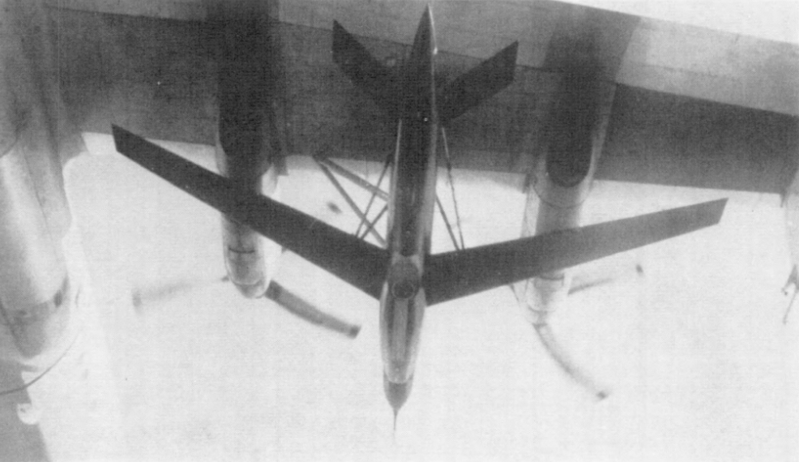
\includegraphics[width=8cm]{./Obrazy/Model_147_RPV.png}
  \caption{Ryan Model 147 Lightning Bug umieszczony pod skrzydłem samolotu transportowego}
  \source{\myurl{https://en.wikipedia.org/wiki/File:Model_147_RPV_pictured_in_flight_under_wing_pylon_of_a_carrier_aircraft.png}}
  \end{figure}

\subsubsection{Ikona wśród BSP}

\hspace{1cm}Zdecydowanie do najpopularniejszego BSP na świecie należy zaliczyć \textit{MQ-1 Predator}. Przez amerykańskiego producenta \textit{General Atomics} jest on klasyfikowany jako zdalnie sterowany statek powietrzny. Pierwsze jego wersje nie posiadały na swoim pokładzie żadnych pocisków, ponieważ amerykanie nie byli pewni czy jest to zgodne z obowiązującym układem dotyczącym całkowitej likwidacji pocisków rakietowych średniego zasięgu (ang. \textit{Intemediate-range Nuclear Forces (INF) Traty}). Po wydarzeniach z 11 września 2001 r. została podjęta decyzja o uzbrojeniu Predatorów w pociski i skierowania ich do akcji. Umożliwiło to prowadzenie operacji militarnych bez ponoszenia strat w żołnierzach. Drony te był wykorzystywane w trakcie konfliktów w Afganistanie, Iraku czy Pakistanie. USA na przestrzeni lat 2009-2021 stało się światowym liderem w używaniu dronów bojowych. \cite{dron-ibuk}\cite{predator-wiki} 


\begin{figure}[!ht]
  \centering
  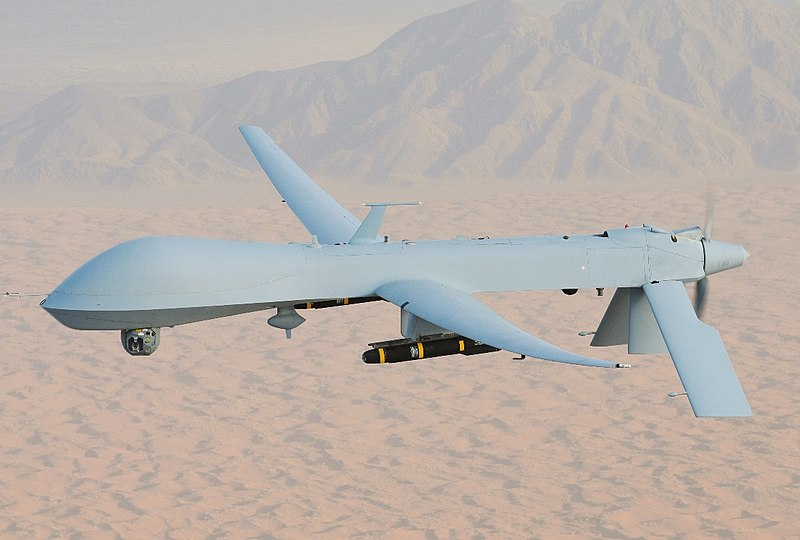
\includegraphics[width=8cm]{./Obrazy/predator.jpg}
  \caption{MQ-1 Predator, wyposażony w rakiety AGM-114 Hellfire}
  \source{\myurl{https://en.wikipedia.org/wiki/File:MQ-1_Predator,_armed_with_AGM-114_Hellfire_missiles.jpg}}
  \end{figure}

\subsubsection{Drony cywilne}
\hspace{1cm}Trudno zaprzeczyć stwierdzeniu, że wojna przyczynia się do szybszego rozwoju, bo to właśnie rozwiązania opracowane dla armii przenoszone są często do życia codziennego. Było tak z herbatą ekspresową, jest tak i teraz z bezzałogowymi statkami powietrznym. Tylko ich rola jest inna, za ich pomocą nie prowadzi się działań wojennych, a nagrywa sceny do filmów czy prowadzi transmisje skoków narciarskich z ciekawszej perspektywy. Drony wyposażone w odpowiednie czujniki powietrza służą też do inspekcji przez zarządy miast, czy obywatele nie spalają w swoich piecach śmieci. Obecny rok można wskazywać jako okres największego zainteresowania tą technologią na rynku cywilnym. Początek tego okresu można próbować określać na 2013 r., czyli datę premiery pierwszej wersji bezzałogowego statku powietrznego \textit{Phantom} od obecnie najpopularniejszego producenta dronów konsumenckich \textit{DJI}.   

\subsubsection{Konfilikt na Ukrainie}
\hspace{1cm}W kontekście bezzałogowych statków powietrznych nie można pominąć aktualnego konfliktu zbrojnego na Ukrainie. Należy go rozpatrywać w dwóch aspektach: przewagi, która armia ukraińska uzyskuje dzięki tureckim dronom \textit{Bayraktar TB2} i wykorzystaniu dronów konsumenckich od ludności cywilnej do przeprowadzenia rozpoznania powietrznego.

Rząd ukraiński zwrócił się z prośbą do swoich obywateli o przekazanie swoich dronów na potrzeby armii. Są one wykorzystywane do bezpiecznego prowadzenie rozpoznania przez wojska ukraińskie. Dostarczają one obraz na żywo, wraz ze swoimi współrzędnymi geograficznymi, pozwala to budować przewagę informacyjną na polu bitwy, a ten konflikt szczególnie uświadomił, jak ważna jest informacja dzisiaj informacja na polu bitwy.\cite{fotografia-drony-ukraina}

Czytając artykuły poświęcone dronom Bayraktar w kontekście konfliktu, można odnieść wrażenie, jakby było to jedyny element budujący ich siłę. Autor nie może się z tym zgodzić, ale nie da się zaprzeczyć, że ich rola jest znacząca. Głównym celem tej maszyny jest prowadzenie rozpoznania, ale mogą być one doposażone w cztery pociski kierowane o zasięgu 8 km. Sam dron jest jedną z tańszych opcji na ryku, bo jego cena wacha się między 2-6 mln dolarów, a drony z najwyższej półki sięgają 100 mln dolarów. Dron o rozpiętości skrzydeł rzędu 12 metrów i 6,5 metra długości może szybować przez 27 godzin lub przelecieć 150 km. Wzbija się na pułap 8200 m i rozwija prędkość do 220 km/h za sprawą silnika \textit{Rotax 912 iS} o mocy 100 koni mechanicznych. \cite{bayraktar-chip}\cite{bayraktar-pap}

\begin{figure}[!ht]
  \centering
  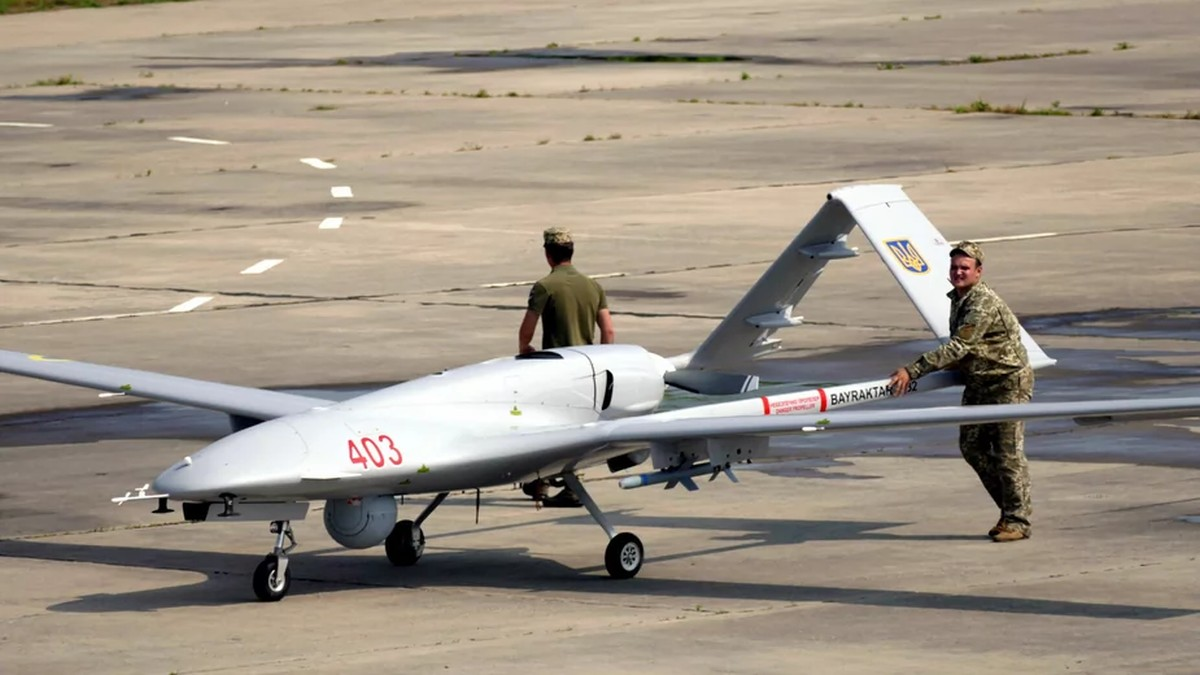
\includegraphics[width=8cm]{./Obrazy/Bayraktar_TB2_ukraina.jpg}
  \caption{Bayraktar TB2}
  \source{\myurl{https://www.instalki.pl/images/newsy/03-2022/Bayraktar_TB2_ukraina.jpg}}
  \end{figure}


\subsection{Technologia i producenci BSP}
\hspace{1cm}Przy porównywaniu producetów dronów należy pamiętać że wymagania stawiane na rynku cywilnym i militarnym znacznie się różnią. Dodatkowo rynek cywilny jest zdominowany przez praktycznie jedno producenta, z militarny z kolei jest za to bardziej zróżnicowany.

\subsubsection{Shenzhen DJI Sciences and Technologies Ltd.}
\hspace{1cm}Shenzhen DJI Sciences and Technologies Ltd., znany powszechnie pod nazwą handlową DJI, jest obecnie największym producentem dronów konsumenckich. Z siedzibą w chińskiej "dolinie krzemowej" Shenzhen.

Firma została założona w 2006 r. , a swój pierwszy sukces odniosła w 2013 r. kiedy wpuściła na ryenk pierwszy model drona \textit{Phantom} Był to BSP przeznaczony dla początkujacych operatorów, a na tle konkurencji wyrózniała go łatwość obsługi. W kolejnych latach firma nadal sie rozwijała, a w 2015 r. wraz z wypuszczeniem trzeciej wersji drona \textit{Phantom} stała się największym producentem na świecie. W 2016 r. firma ta posiadała 50\% udziałow w światowym rynku, a rok pózniej już 72\%. W 2020 r. było około 74\%, podczas gdy żadna inna firma w tym samym czasie nie posiadała więcej niż 5\% udziału w światowym rynku.\cite{dji-wiki}\cite{dji-market-share}

W 2020 r. BSP firmy DJI były wykorzystane przez Chiny do przypominania ludzią o obowiązku noszenia maseczek na twarzy w celu ograniczenia rozprzestrzeniania sie wirsua COVID-19. Z tego samego powodu w takich krajach jak Maroko czy Arabia Sudyjska drony mierzyły temperatury przmieszczającającej sie populacji w teranach silnie zurbanizowanych.

\subsubsection{Yuneec International}

\hspace{1cm}Yuneec International to drugi największy producent dronów konsumenckich, w rynku światowym posiada zaledwie 5\% udziałow. Firma ta została założona w 1999 r., a jej obecna siedziba znajduje się w Jiangsu w Chinach.

\subsection{Zastosowania BSP}
\hspace{1cm}Bezpilotowe statki latające znalazły szereg zastosowań, pierowotnie były wykorzystywane głównie w obszarze militarnym, dopiero później dostrzegł w nich potencjał obszar cywilny.  

\subsubsection{Militarne zastosowania BSP}
\hspace{1cm}Bezałogowe statki powietrzne w kontekście militarnym można dokonać podziąłu na następujące kategorie \cite{konkurs-mon}: 
\begin{itemize}
  \item \textbf{operacyjno-rozpoznawcze}: BSP umożliwiające, rozpoznawanie oraz śledzenie obiektu/celu, a także monitorowanie i kontrole obszaru zainteresowania, np. granic lub strefy przybrzeżnej. Przykładem takieg dronu jest Lockheed Martin RQ-170 Sentinel;
  \item \textbf{bojowe}: BSP przenoszącce i używające środki bojowe/ środki rażenia np. Bayraktar TB2;
  \item \textbf{amunicja krążąca}: BSP umożliwijące wykrywanie, rozpoznanie oraz atak na wyznaczony cel poprzez autodestrukcje np. WB Electronics Warmate;
  \item \textbf{wsparcia}: BSP umożliwiające ewakuacje lub dostawe amunicji, wyposażenia, środków medycznych i żywności do wysuniętych stanowisk wojsk własnych. np. Kaman KARGO UAV 
\end{itemize}

\subsubsection{Rolnictwo}
\subsubsection{Transport towarów i osób}
\subsubsection{Kinematografia i transmisje sportowe}
\subsubsection{Ratownictwo}

\hspace{1cm} http://han.wat.edu.pl/han/ibuk/https/libra.ibuk.pl/reader/drony-wprowadzenie-technologie-zastosowania-sarah-e-kreps-203891

\hspace{1cm}text
\subsection{Dostosowywanie drona do wymagań użytkownika}
\hspace{1cm}text

\newpage 
\section{Przegląd i prezentacja technologii mobilnych z uwzględnieniem aspektów tworzenia aplikacji i komunikacji M2M}
\hspace{1cm}W tym rozdziale przedstawiono technologie komunikacji bezprzewodowej wykorzystywane w komunikacji M2M, ze szczególnym uwzględnieniem komunikacji pomiędzy bezzałogowym statkiem powietrznym, a kontrolerem. Analizę wykorzystywanych rodzajów komunikacji dokonano na podstawie oferty najpopularniejszego producenta dronów konsumenckich DJI.

\subsection{Komunikacja M2M}
\hspace{1cm}Komunikacja M2M (machine-to-machine) służy do definiowania technologi, która umożliwia wymianę informacje pomiędzy urządzeniami w sieci bez jakikolwiek ingerencji ludzi. Sztuczna inteligencja wraz z metodami uczenia maszynowego znacznie ułatwia takie procesy, między innymi umożliwia ona podejmowanie autonomicznych decyzji przez te urządzenia. Ta komunikacja jest podstawą istnienia IoT.\cite{m2m-web}

\subsubsection{Cel}
\hspace{1cm}Głównym celem M2M jest przenoszenia danych z sensorów do sieci. W porównaniu do innych technolgi, które umożliwiają monitorowanie zasobów, korzysta ona często z dostępnych publicznie sieci np. GSM, co redukuje jej koszty utrzymania. Można wyróżnić 3 elemnty takiego systemu:
\begin{itemize}
  \item łącze do przesyłu danych, np. WiFi, GSM, RFID
  \item sensory, np. czujnik temperatury, kamera
  \item oprogramowaie, które umożliwia podejmowanie zautmatyzowanych decyzji
\end{itemize}
\hspace{1cm}Najpopularniejszą dziedziną tej technologii, jest telemetria. Jej celem jest pomiar wybranej wielkości i jej przesyłanie do centralnej jednostki, oddalonej od miejsca pomairu. Na początku do tego celu były wykorzystywane linie telefoniczne, a następnie radiowe. Rozwój technologi, a w tym łączności bezprzewodowej sprawił, że rola wykorzystywania telemetrii w nauce inżynierii i produkcji poszerzyła się do użytku codziennego w jednostkach grzewczych, mierników elektrycznych i wszelkich urządzeń podłączonych do internetu.\cite{m2m-web}

\subsubsection{Wymagania}
\hspace{1cm}Według Europejskiego Instytutu Norm Telekomunikacyjnych (ETSI) komunikacja M2M musi spełniać następujące wymagania:
\begin{itemize}
  \item \textbf{Skalowalność}: w miarę dołączania kolejnych urządzeń do systemu system nadal musi funkcjonować;
  \item \textbf{Anonimowość}: na każde żądanie, w związku z wymaganiami prawnymi system musi umożliwiać ukrywanie tożsamości urządzenia;
  \item \textbf{Logowanie}: ważne wydarzenia w systemie, takie jak: pojawienie się błędnych informacji czy nieudane próby instalacji, muszą być zarejestrowane, a rejestry te muszą być dostępne na żądanie;
  \item \textbf{Zasady komunikacji między aplikacjami}: aplikacje w systemie powinny mieć możliwość komunikowania się. W szczególności bramki i urządzenia końcowe komunikujące się za pomocą technologi SMS czy Ethernet powinny komunikować
  się za pomocą połączenia P2P (peer-to-peer);
  \item  \textbf{Metody dostarczania}: w ramach systemu powinny być dostarczane metody komunikacji takie jak: \emph{unicast}, \emph{multicas}, \emph{broadcast} i \emph{annycast}, a wszędzie gdzie to możliwe metoda \emph{broadcast} powinna być zastąpiona za pomocą \emph{multicast}, tak aby zminimalizować obciążenie sieci;
  \item \textbf{Harmonogram przesyłania komunikatów}:  dostęp do sieci powinien być kontrolowany, tak samo, jak harmonogram przesyłania komunikatów. Sam system powinien również uwzględniać obciążenia aplikacji M2M w harmonogramie przesyłania wiadomości;
  \item \textbf{Wybór ściezek komunikacjynych}: ścieżki w systemie powinny zapewniać optymalizacje bazującą na: awariach transmisji, kosztu i opóźnieniach, w momencie, gdy istnieją inne ścieżki do punktu docelowego. \cite{m2m-web}
\end{itemize}

\subsection{Technologie komunikacji M2M}
\hspace{1cm}Gdyby w technologi tak samo, jak w literaturze występowały epoki, aktualnie znajdowalibyśmy się w epoce połączonych ze sobą obiektów. IoT (Internet of Things) zdobywa aktualnie coraz więcej uwagi nie mal w każdej domenie, a szczególnie w takich jak biznes, elektronika konsumencka, przemysł czy transport. Niemal każdy obiekt elektryczny w dzisiejszym świecie jest ze sobą połączony w ten czy inny sposób. Siedząc w biurze, za pomocą dostarczanych aplikacji, możemy kontrolować drzwi, bramę garażową, czajnik elektryczny czy rolety okienne w naszym domu. W mieście kontrolujemy kamery i oświetlenie z odległych lokacji. IoT odgrywa w tym ważną rolę, ponieważ to ono umożliwia łączenie przeróżnych obiektów, za pomocą sieci połączeń i wymianę danych między nimi.\cite{LoRa-article}

\subsubsection{Ogólna klasyfikacja technolgi M2M}
\hspace{1cm}Poniżej przedstawiono ogólne porównanie technologi komunikacyjnych M2M.

\begin{table}[!htbp]
  \resizebox{\textwidth}{!}{%
  \begin{tabular}{|l|l|l|l|}
  \hline
  \textbf{}            & \begin{tabular}[c]{@{}l@{}}\textbf{Local Area Network}\\ Komunikacja krótko \\ dystansowa\end{tabular}            & \begin{tabular}[c]{@{}l@{}}\textbf{Low Power Wide Area}\\ Intenet Of Things\end{tabular}            & \begin{tabular}[c]{@{}l@{}}\textbf{Celluar Network}\\ Tradycyjne M2M\end{tabular}                               \\ \hline
  \textbf{Użycie}      & 40\%                                                                                                              & 45\%                                                                                                & 15\%                                                                                                            \\ \hline
  \textbf{Zalety}      & \begin{tabular}[c]{@{}l@{}}- Dobrze ugruntowana norma\\ - W budynkach\end{tabular}                                & \begin{tabular}[c]{@{}l@{}}- Niskie zużycie energi\\ - Niskie koszty\\ - Pozycjonowanie\end{tabular} & \begin{tabular}[c]{@{}l@{}}- Istniejące pokrycie znacznego \\ obszaru\\ - Duża prędkość transmisji\end{tabular} \\ \hline
  \textbf{Wady}        & \begin{tabular}[c]{@{}l@{}}- Wysokie zużycie energi \\ elektrycznej\\ - Duży koszt sieci i zależności\end{tabular} & \begin{tabular}[c]{@{}l@{}}- Niska prędkość transmisji\\ - Wschodzący standard\end{tabular}         & \begin{tabular}[c]{@{}l@{}}- Wysoki koszt posiadania\\ - Mała autonomia\end{tabular}                            \\ \hline
  \textbf{Technologia} & Bluetooth, WiFi                                                                                                   & LoRa                                                                                                & GSM, 3G, 4G, 5G                                                                                                 \\ \hline
  \end{tabular}%
  }
  \caption{Porównanie rodzajów technolgi M2M.\cite{LoRa-article}}
\end{table}

\subsubsection{LoRa}
\hspace{1cm}LoRa (Long Range) to nowa technologia połączeń bezprzewodowych w świecie IoT, która ostatnio ewoluowała i zyskała szczególną popularność, w urządzeniach z ograniczoną pojemnością elektryczną umożliwiając systemom wbudowanym przesyłanie małej ilości danych na dużych dystansach w krótkich interwałach czasowych.

\hspace{1cm}Komunikacja w aplikacjach IoT jest dzisiaj wykonywana w przeróżnych technologiach, a każda z nich ma swoje zalety, funkcje, a przez to też przeznaczenie. Żadna z tych technolgi nie może pokryć całego zapotrzebowania świata IoT, ponieważ wszystkie one posiadają cechy, które czynią je odpowiednie dla postawionego konkretnego zadania.

\hspace{1cm}WiFi to najpopularniejsza technologia komunikacji bezprzewodowej, która ewoluowała przez wiele lat i jest wykorzystywana przede wszystkim do komunikacji na dużych
odległościach. Na krótkie dystanse mamy przeznaczone do tego no. Bluetooth czy ZigBee. We wszystkich z nich największą wadą jest duże zużycie energii elektrycznej. Technologia Lora zapewnia bezpieczne, mobilne dwukierunkowe połączenie o niskim koszcie elektrycznym, wykorzystywane jest ono w IoT, szczególnie w domenie smart city, czy nawet ogólnej komunikacji M2M. LoRa zalicza się do LPWA(Low Power Wide Area), czyli rodzaju bezprzewodowej rozległej sieci telekomunikacyjnej, stworzonej w celu umożliwienia komunikacji na duże odległości przy niskiej przepływności i niskim poborze energii. \cite{LPWA-wiki} W tego typu komunikacji wyróżnia się LoRa ze względu na jej:
\begin{itemize}
  \item długodystansowość;
  \item dwukierunkowość;
  \item wysoką pojemność węzłów w sieci;
  \item długość życia na baterii;
  \item odporność interfejsów;
  \item bezpieczeństwo i efektywność sieci. \cite{LoRa-article}
\end{itemize}


\myparagraph{Cechy}
\hspace{1cm}Technologie tą wyróżniają następujące cechy:
\begin{itemize}
  \item Pojedyncza bramka może pokryć obszar aż $100km^2$;
  \item Oferuje ona podwójne szyfrowanie AES;
  \item Bazuje na technologi CSS (widmo rozproszone Chrip), które umożliwia śledzenie obiektów i jest odporne na zanikanie sygnałów;
  \item Topologia gwiazdy eliminuje zanikanie danych przez urządzenia pośrednie, co przyczynia się do zmniejszenia poboru mocy. \cite{LoRa-article}
\end{itemize}


\myparagraph{Ograniczenie przepustowości}
\hspace{1cm}W sieci LoRa wszystkie klasy ramek wymagają potwierdzenia, co wiąże się z tym, że po każdym potwierdzeniu ramko przez urządzenie końcowe w dowolnym oknie czasowym następuje okres wyłączenie, w celu zachowanie zgodności z przepisami dotyczącymi cyklu pracy. W związku z tym, aby uniknąć wyczerpania limitu pojemności przez sieć i urządzenia końcowe, muszą one ograniczyć liczbę potwierdzeń. Również w podsieciach LoRa po przesłaniu danych następuje okres wyłączenia, w którym na danym kanale nie są wysyłane żadne dane. Te dwa okresy, tzn. okres wysyłania danych i wstrzymania transmisji stanowi cykl pracy, dlatego  to w sieci LoRa przepustowość jest ograniczona cyklem pracy.\cite{LoRa-article}

\subsubsection{Narow band IoT}
\hspace{1cm}Wraz z rozwojem świata IoT NB-IoT stało sie wiodącą technologią komunikacji komórkowej dla zdalnych pomiarów w całej Europie. NB-IoT to technologia dostępu radiowego, która ponownie używa komponentów stworzonych przez jej poprzednika LTE, aby umożliwić jej działa na licencjonowanej częstotliwości. Może ona również działać w trybie autonomicznym. Tak jak sama nazwa wskazuje, cały system działa w wąskim spektrum częstotliwości, bo tylko w 200kHz, co wprowadza elastyczność zastosowań dzięki minimalnym wymaganiom częstotliwości, w porównaniu do jej poprzednika LTE. Cała szerokość 200kHz została podzielona na kanały po 3.75 kHz lub 15 kHz, co umożliwia połączenie w bardzo wysoką prędkość nadawania, a także daleki zasięg połącznika, biorąc pod uwagę wąskie widmo sygnału. \cite{nbiot-article}  

\subsubsection{NB-IoT vs Lora}

\begin{table}[!htbp]
  \resizebox{\textwidth}{!}{%
  \begin{tabular}{|l|c|c|}
  \hline
  \textbf{Parametr}                                                                     & \textbf{LoRa}               & \textbf{NB-IoT}       \\ \hline
  \textbf{Pasmo}                                                                        & 125 kHz                     & 180 kHz               \\ \hline
  \textbf{Pokrycie}                                                                     & 165 dB                      & 164 dB                \\ \hline
  \textbf{Żywotność baterii}                                                            & 15+ lat                     & 10+ lat               \\ \hline
  \textbf{\begin{tabular}[c]{@{}l@{}}Maksymalne natężenie \\ elektryczne\end{tabular}}  & 32 mA                       & 120 mA                \\ \hline
  \textbf{\begin{tabular}[c]{@{}l@{}}Spoczynkowe natężenie \\ elektryczne\end{tabular}} & 1 µA                        & 5 µA                  \\ \hline
  \textbf{Przepustowość}                                                                & 50 Kbps                     & 60 Kbps               \\ \hline
  \textbf{Opóźnienie}                                                                   & Zależne od klasy urządzenia & 10 s                  \\ \hline
  \textbf{Bezpieczeństwo}                                                               & AES 128 bit                 & 3GPP (128 to 256 bit) \\ \hline
  \textbf{Geolokalizacja}                                                               & Tak (TDOA)                  & Tak (In 3GPP Rel 14)  \\ \hline
  \textbf{Jakość/cena}                                                                  & Wysoka                      & Średnia                \\ \hline
  \end{tabular}%
  }
  \caption{Porównanie technologi LoRa i NB-IoT \cite{NB-IoT_vs_Lora}}
  \end{table}

\hspace{1cm}Zarówno LoRa jak i NB-IoT należą do wspomnianej wcześniej technologi LPWAN. Podstawowa różnice pomiędzy tymi dwoma technologiami można dostrzec w zużyciu baterii, prędkości transmisji i opóźnień.

\subsection{Komunikacja bezprzewodowa w dronach konsumenckich}
\hspace{1cm}Przeglądając katalog największego producenta dronów konsumenckich DJI, można wyróżnić tylko 3 technologie komunikacji bezprzewodowej: wzomocnione WiFi (ang. enhanced WiFi), Lightbridge, OcuSync.

\subsubsection{WiFi}
\hspace{1cm}WiFi nie zostało wprowadzone ściśle do komunikacji bezprzewodowej statków powietrznych, ale odnajduje się w tym całkiem dobrze. Jest ona wykorzystywana głównie w bardziej budżetowych wersjach dronów, ze względu na możliwość skorzystanie przez producenta z posiadanej przez użytkownika infrastruktury (smartfonów), czy niskiej ceny komponentów.

\hspace{1cm}Przykładowo dron \emph{DJI Tello}, który jest najtańszą opcją dostępną od producenta DJI, przeznaczoną głównie do nauki latania, a nawet praktycznie programowania przez najmłodszych pasjonatów, nie posiada on w zestawie dedykowanego kontrolera. Kontrolowanie drona odbywa się za pomocą aplikacji na smartfona, która łączy się z dronem za pomocą WiFi tak jak do punktu dostępowego z internetem. Zasięg takiego połączenia według producenta to 100m \cite{dji-store}.


\begin{figure}[!htbp]
  \centering
  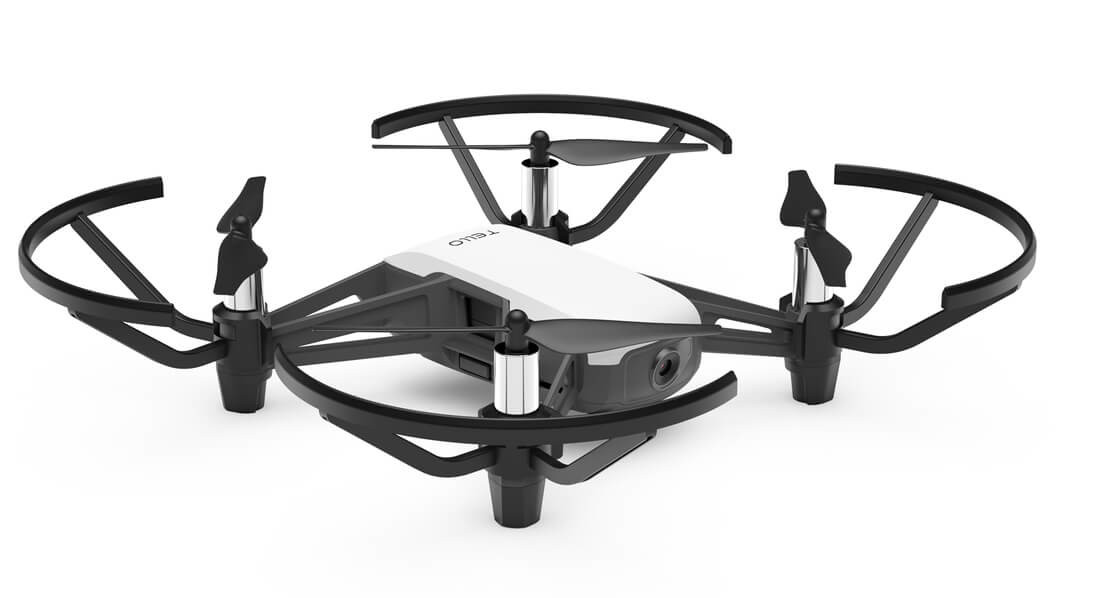
\includegraphics[width=10cm]{./Obrazy/dji-tello.jpg}
  \caption{DJI Tello}
  \source{\myurl{https://store.dji.com}}
  \end{figure}

\hspace{1cm}W swojej ofercie DJI ma również dostępnego drona \emph{DJI Mini SE}, który również korzysta z technologii WiFi, ale w swoim wyposażaniu posiada dedykowany do niego kontroler. Taka konfiguracja pozwala na uzyskanie zasięgu do 2 km. \cite{dji-mavic-mini-se-spec}

\hspace{1cm}WiFi jest także bardzo podatne na wszelkie zakłócenia, wynikające z ukształtowania terenu czy zaszumienia sieci pochodzącego z istniejących sieci domowych. Wyprodukowanie drona w tej technolgi jest najtańszą dostępną opcją, która umożliwia transmisje obrazu, jednak należy pamiętać, aby nie stawiać jej przy tym za dużych wymagań. WiFi stanowi bardzo dobry punkt startowy w komunikacji bezprzewodowej bezzałogowych statków powietrznych.

\subsubsection{Lightbridge}
\hspace{1cm}Lightbridge to technologia od DJI, która doczekała się jej dwóch wydań. Pierwszych wzmianek o niej można doszukiwać się w 2014 roku. \cite{lightbridge-dji}, a drugiego wydania już w 2015 roku\cite{lightbridge2-dji}. Obecnie nie jest już rozwijana, a producent skupił się na rozwoju jego drugiej technologi: OcuSync.

\hspace{1cm}Technologie prezentowane przez DJI mają parę cech zbliżające je do WiFi, przede wszystkim transmisja ta odbywa, gdyż odbywa się ona na tej samej częstotliwości: 2,4GHz. Była ona kierowana głównie do dronów z wyższego pułapu cenowego, dlatego że jej produkcja była bardzo kosztowna, a koszt wynikał z tego, że producent opracował to rozwiązanie na swoim autorskim układzie scalonym i oprogramowaniu. Wskutek czego pozwoliło to osiągnąć duże lepsze wyniki niż transmisja po WiFi. Zasięg lotu według producenta to odległość do 5km.

\subsubsection{OcuSync} 
\hspace{1cm}OcuSync został po raz pierwszy zademonstrowany przez producenta wraz z wydaniem drona \emph{Mavic Mini Pro}. Pierwsze wydanie tej technologi pozwalało na transmisje do 7km na częstotliwości 2,4GHz. Obraz mógł być przesyłany w rozdzielczości 720p i 1080p. Jakość fullHD była dostępna tylko na krótszych odległościach, gdy dystans się zwiększał, a dostępna prędkość transmisji spadała, dron przechodził automatycznie na transmisje w 720p. Opóźnienie było rzędu 160-170ms. A największą cechą wyróżniającą tę technologię była możliwość podłączenia jednocześnie dwóch kontrolerów i do 4 urządzeń odbiorczych.

\hspace{1cm}Kolejnym krokiem było wydane kolejnej wersji oznaczonej jako OcuSync 1.5, w której dodano transmisję również na częstotliwości 5Ghz. Zmniejszono także opóźnienia w transmisji. Dodatkowo technologia umożliwiał automatyczną zmianę kanałów komunikacyjnych w trakcie lotu na te najmniej obciążone. W pierwszej wersji kanał 
transmisji można było wybrać tylko przed startem bezzałogowego statku powietrznego.


\begin{figure}[!ht]
  \centering
  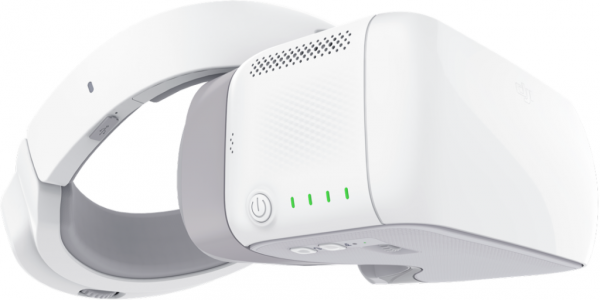
\includegraphics[width=8cm]{./Obrazy/dji-google.png}
  \caption{Pierwsza wersja gogli do FPV od DJI}
  \source{\myurl{https://u.cyfrowe.pl/600x0/2/7/2_732250420.png}}
  \end{figure}
  

\begin{figure}[!ht]
  \centering
  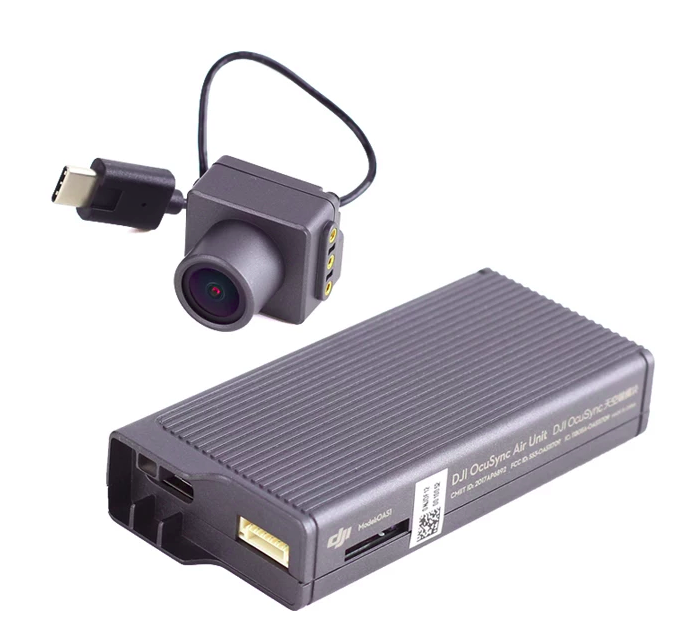
\includegraphics[width=8cm]{./Obrazy/dji-air-unit.png}
  \caption{Dji OcuSync Air Unit}
  \source{\myurl{https://store.dji.com}}
  \end{figure}

\hspace{1cm}Wraz z wydaniem nowej wersji zaprezentowano gogle DJI przeznaczone do transmisji obrazu w trybie FPV (ang. first person view, widok pierwszo-osobowy) i również OcuSync Aircraft System, czyli zintegrowanego systemu umożliwiającego sterowanie i transmisji obrazu z wykorzystaniem tej technologi w dronach i pojazdach DIY.

\hspace{1cm}Producent w trakcie swojej historii doprowadził do pewnych nieścisłości, mimo że dron \emph{Phantom 4 pro v 2.0} korzystał teoretycznie z najnowszej wersji OcuSync, ale nie posiadał on możliwości zmiany kanałów transmisji w trakcie lotu, opóźnienie zależało też od tego, czy korzystano z kontrolera dołączonego do zestawu, czy jego droższej, lepiej wyposażonej wersji: \emph{DJI RC Plus}.
  

\begin{figure}[!ht]
  \centering
  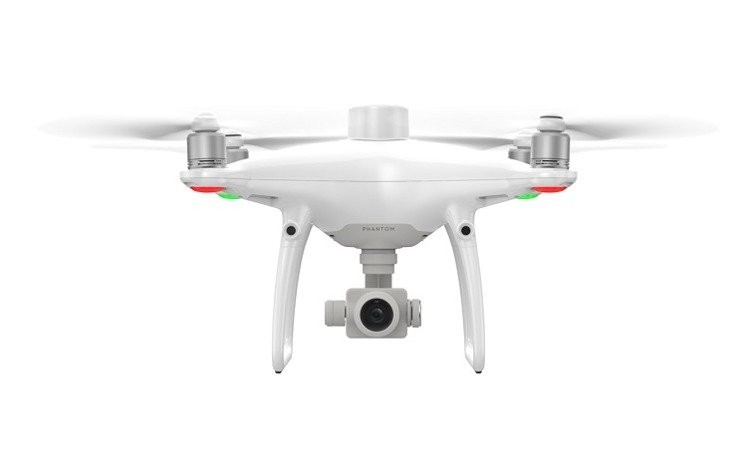
\includegraphics[width=8cm]{./Obrazy/dji-phantom-v2.jpg}
  \caption{DJI Phantom v2.0}
  \source{\myurl{https://store.dji.com}}
  \end{figure}
  

\begin{figure}[!ht]
  \centering
  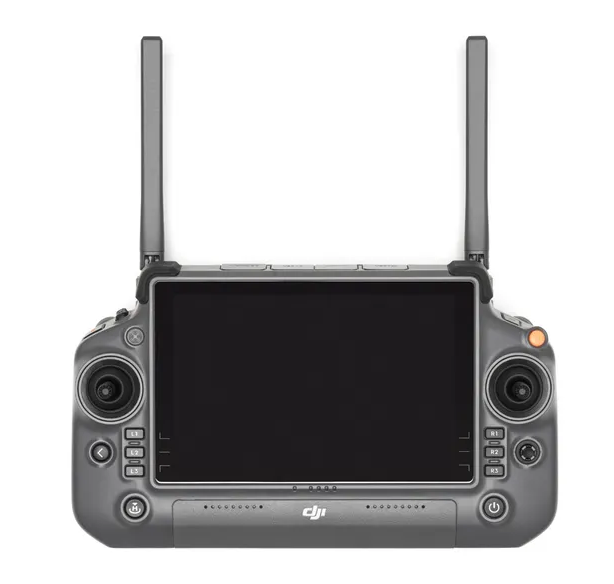
\includegraphics[width=8cm]{./Obrazy/dji-rc-plus.png}
  \caption{DJI RC plus}
  \source{\myurl{https://store.dji.com}}
  \end{figure}
  


\hspace{1cm}Wersja 2.0 wprowadziła dalsze ulepszenia, m.in. kontorlowanie dronów na jeszcze większe dystanse i z jeszcze mniejszymi opóźnieniami, a także kompatybilność wsteczną po aktualizacji oprogramowania.

\newpage
\subsubsection{FHSS i  OFDM}

\hspace{1cm}Zarówno Lightbridge, jak i OcuSync używają szyfrowanej modulacji OFDM (ang. Orthogonal Frequency-Division Multiplexing, zwielokrotnianie z ortogonalnym podziałem częstotliwości)) dla transmisji obrazu i z formy FHSS (ang. Frequency-Hopping Spread Spectrum) dla transmisji sygnałów sterowania. Kanał dla transmisji obrazu nie zmienia się w trakcie całego lotu, pod warunkiem, że nie następują zakłócenia, albo użytkownik nie ustawi ręcznie innej częstotliwości. Z kolei metoda FHSS "skacze" po częstotliwościach w całym dostępnym widmie, w tym nawet w pasmie przenzaczonym do transmij obrazu.\cite{FHSS-wiki} \cite{OFDM-wiki}

\begin{figure}[!htbp]
\centering
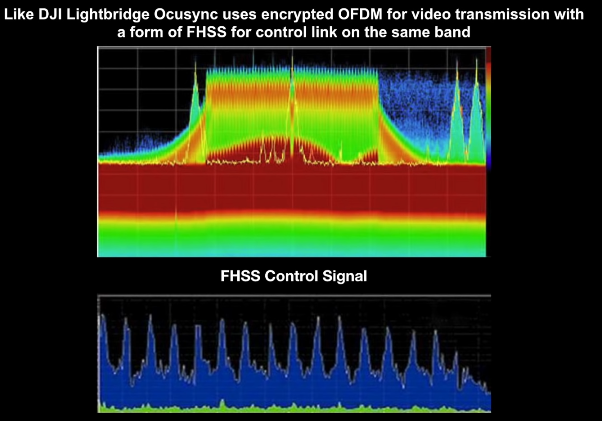
\includegraphics[width=14cm]{./Obrazy/ocusync_spectrum_1.png}
\caption{Widmo OFDM i FHSS}
\source{\myurl{https://www.youtube.com/watch?v=gfqcSv9sR0A}}
\end{figure}

\begin{figure}[!htbp]
\centering
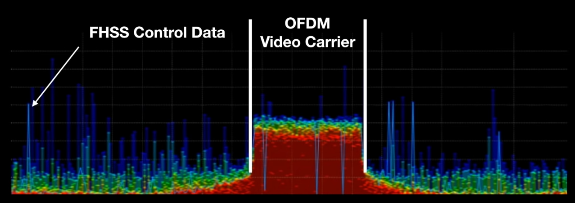
\includegraphics[width=14cm]{./Obrazy/ocusync_spectrum_2.png}
\caption{Widmo OcuSync z zaznaczoną modulacja FHSS i OFDM}
\source{\myurl{https://www.youtube.com/watch?v=gfqcSv9sR0A}}
\end{figure}


\begin{figure}[!htbp]
\centering
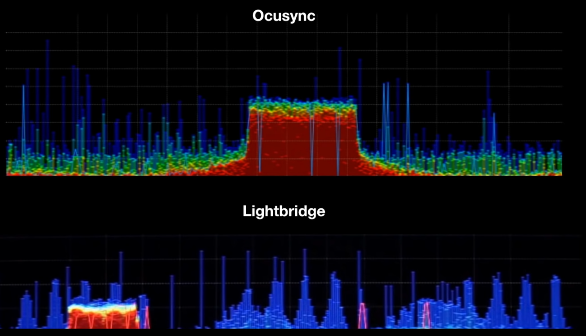
\includegraphics[width=14cm]{./Obrazy/ocusync_vs_lightbridge.png}
\caption{Porównanie widma OcuSync i Lightbridge}
\source{\myurl{https://www.youtube.com/watch?v=gfqcSv9sR0A}}
\end{figure}

\newpage

\subsubsection{Przewaga OcuSync nad Lightbridge}
\hspace{1cm}OcuSync stało się główną technologią rozwijaną przez DJI, ponieważ wykorzystuje ono istniejące układy scalone przeznaczone do komunikacji WiFi. Producent wytwarza na nie swoje własne oprogramowanie, które możne następnie aktualizować. Lightbridge był ich własnym układem scalonym, którego oprogramowania nie można było aktualizować, w dodatku komunikacji opierała się wyłącznie na paśmie 2,4GHz. Nowe procesory w układach WiFi dzięki coraz większej częstotliwości pracy zapewniły osiąganie tych samych efektów co Lightbridge, bez dodatkowego kosztu wynikającego z produkcji własnego układu scalonego. 

\subsection{Sterowanie dronami za pomocą API dostarczaonego od producenta}
\hspace{1cm}Przeszukując internet w poszukiwaniu bezzałogowych statków powietrznych umożliwiających ich sterowanie za pomocą API od producenta można napotkać głównie rozwiązania od DJI. Wszystkie pozostałe rozwiązania nie działają na gotowych dronach, a na oprogramowaniu przeznaczonym do wgrania na wybranych jednostkach do sterowania  modelami RC. 

\hspace{1cm}Najpopularniszym tego rozwiązaniem jest ArduPilot, czyli pakiet oprogramowania nawigacyjnego działającego w pojezdie wraz z oprogramowaniem sterującym stacją naziemną. 

\subsubsection{DJI SDK}
\hspace{1cm}DJI dostarcza do swoich produktów następujące interfejsy API:
\begin{itemize}
  \item \textbf{App Dev.} - interfejsy API przeznaczone do sterowania dronem z poziomu stacji bazowej, kontroler stanowi interfejs pośredniczący między aplikacją wykorzystującą SDK a dronem powietrznym:\begin{enumerate}
    \item \textbf{Mobile SDK} - SDK przeznaczona na platformę iOS i Android. Aplikacja na smartfon za pomocą kabla USB podłączonego do kontrolera statku powietrznego realizuje zaprogramowaną logikę działania.
    \item \textbf{UX SDK} - Mobile SDK rozszerzony o elementy interfejsu użytkownika, co przyspiesza znacznie proces tworzenia oprogramowania.
    \item \textbf{Windows SDK} - SDK umożliwiające wydawanie aplikacji na systemach operacyjnych Windows. 
  \end{enumerate}
  \item \textbf{Payload Dev.} - interfejsy API przeznaczone do nadawania logiki działania drona na poziomie samego drona, dzięki temu po utracie zasięgu może ona dalej funkcjonować zgodnie z zaprogramowaną logiką. Opcja dostępna dla najdroższych wersji dronów DJI, które można dostosowywać do swoich wymagań za pomocą odpowiednich rozszerzeń, np. kamery termowizyjnej\begin{enumerate}
    \item \textbf{Payload SDK} - zestaw narzędzi programistycznych umożliwiających tworzenie oprogramowania do rozszerzeń, które mogą być montowane na dronach DJI. 
    \item \textbf{Onboard SDK} - otwarto źródłowa umożliwiająca komunikacje bezpośrednia z wybranymi dronami i kontrolerami za pomocą interfejsu szeregowego.  
  \end{enumerate}
\end{itemize}

\newpage
\section{Projekt mobilnego systemu zarządzania i sterowania BSP}
\subsection{Wymagania funkcjonalne}
\hspace{1cm}text
\subsection{Wymagania pozafunkcjonalne}
\hspace{1cm}text
\subsection{Stos technologiczny}
\hspace{1cm}text
\subsubsection{Java}
\hspace{1cm}text
\subsubsection{Kotlin}
\hspace{1cm}text
\subsubsection{DJI Mobile SDK}
\hspace{1cm}text
\subsubsection{Lombook}
\hspace{1cm}text
\subsubsection{Springboot}
\hspace{1cm}text
\subsubsection{Android}
\hspace{1cm}text
\subsection{Uzasadnienie warstwy pośredniczącej}
\hspace{1cm}text
\subsection{Wysokopoziomowy diagram systemu}
\hspace{1cm}text
\subsection{Diagram komponentów}
\hspace{1cm}text
\subsection{Diagram klas i sekwencji}
\hspace{1cm}text
\subsubsection{Gradle}
\hspace{1cm}text
\subsection{Wykorzystane urządzenia}
\hspace{1cm}text

\newpage
\section{Implementacja systemu}
\hspace{1cm}text

\newpage
\section{Testy systemu oraz prezentacja użycia na wybranym case study}
\hspace{1cm}text
\subsection{Scenariusz testowy autonomicznego lotu pomiędzy dwoma punktami}
\hspace{1cm}text
\subsection{Scenariusz testowy autonomicznego lotu patrolowego}

\newpage
\section{TMP}

\subsection{Tytuł podrozdziału}
W procesie dyplomowania tekst pracy jest przetwarzany elektronicznie za pośrednictwem systemów USOS APD (Archiwum Prac Dyplomowych) oraz JSA (Jednolity System Antyplagiatowy). Plik pracy zapisany w formacie ,,pdf'' winien mieć nazwę nadana wg schematu: \textit{,,WAT, myślnik, numer indeksu studenta, myślnik, data wysłania w formacie dd-mm-rrrr''}, np. \textit{,,WAT-12345-01.05.2021.pdf''}. Plik umieszczany jest w systemie USOS APD poprzez indywidualne konto Dyplomanta.

Do pracy można załączyć dodatkowe pliki w formacie ,,docx''/,,pdf''.`'
W przypadku innych formatów (w tym „zip”) , należy je zapisać na płycie CD/DVD, opisanej trwale (niezmywalnym mazakiem) następująco: skrót nazwy uczelni, nazwa wydziału, kierunek studiów, specjalność, numer albumu studenta, imię i nazwisko studenta, temat pracy dyplomowej, własnoręczny podpis studenta. 

\subsection{Tytuł podrozdziału}

W tekście pracy kolejne wątki tematyczne należy oddzielać poprzez wcięciami akapitowe. W strukturze pracy zalecane jest:
\begin{itemize} 
    \item w przypadku wprowadzenia podrozdziałów wyróżnienie co najmniej dwóch na danym poziomie zagłębienia.
\end{itemize}

Praca powinna zawierać oryginalny tekst. W przypadku cytowania należy stosować przypisy dolne. W przypadku odwołania do literatury lub źródeł internetowych należy wstawiać hiperłącza do odpowiednich pozycji z bibliografii, np. [1].
 
Wszystkie skróty w pracy przy pierwszym ich użyciu powinny być rozwinięte (wyjaśnione). Pojedyncze litery z końca wierszy powinny być przeniesione na początek kolejnych wierszy poprzez wprowadzenie tzw. ,,twardej spacji'' pomiędzy tą literą a kolejnym wyrazem (np. w edytorze Microsoft Word poprzez kombinację klawiszy Ctrl+Shift+Spacja).

Pracę mogą kończyć spisy rysunków i tabel – zalecane jest ich wprowadzenie w przypadku wystąpienia dużej liczby rysunków lub tabel w tekście pracy (powyżej 10). Praca może być uzupełniona załącznikami. W przypadku braku w pracy spisów rysunków i tabel lub załączników należy usunąć je ze struktury pracy oraz spisu treści.

Dla tekstu, tytułów, podpisów należy stosować style Wydziału (docx) lub zdefiniowane w~tym szablonie.\\
Układ marginesów i numerów stron przewidziany jest do wydruku dwustronnego.\\
Wydruk pracy nie jest wymagany.


Tabele i rysunki należy wyśrodkować. Dla podpisów stosowane są style Wydziału (docx) lub otoczenie table i tabular oraz figure (LaTeX):
\begin{itemize}
    \item Nazwa tabeli umieszczona ponad tabelą;
    \item Podpis rysunku umieszczony pod rysunkiem;
    \item Źródło rysunku lub danych w tabeli pod tabelą/rysunkiem.
\end{itemize}
Numeracja tabel i rysunków powinna być ciągła i automatyczna w całej pracy.
\begin{table}[H]
    \caption{Nazwa tabeli}
    \label{tab1}
    \begin{center}
        \begin{tabular}{|c|c|c|c|}
                \hline
                \textbf{Lp}     & \textbf{Kolumna 1}    & \textbf{Kolumna 2}    & \textbf{Kolumna 3}    \\ \hline
                1.              & Zawartość tabeli      & Zawartość tabeli      & Zawartość tabeli   \\ \hline
        \end{tabular}
    \end{center}
    \source{Badania własne. Jeżeli dane pochodzą z literatury lub zasobów sieci Internet, należy podać ich źródło. W~innym przypadku można podać: Badania własne.}
\end{table}

Dla wzorów zaleca się stosować wyśrodkowanie. Numerację automatyczną ciągłą w~całej pracy należy wyrównać do prawej strony – przykład poniżej:
\begin{equation}
    \label{eq1}
    \displaystyle \sum_{j=0}^{n}a_{ij} \leq 1, i = \overline{1, n}
\end{equation}

Kod źródłowy oraz algorytmy umieszcza się w tabelach dwukolumnowych (docx), lub otoczenia lstlisting i algorithm (LaTeX), z numeracją wierszy w pierwszej kolumnie:
\begin{itemize}
    \item Tekst w tabeli kodu źródłowego: czcionka Courier New 11 pkt., wyjustowany do lewej;
    \item Nazwa kodu źródłowego umieszczona ponad kodem;
    \item Nazwa algorytmu umieszczona ponad algorytmem;
    \item Źródło kodu lub algorytmu poniżej.
\end{itemize}

\begin{lstlisting}[language=Verilog, caption=Nazwa kodu źródłowego \label{TbECMont}]
    int silnia (int a)
    {
        return (a == 1) ? a : a * silnia(a-1);
    }
\end{lstlisting}
\source{Badania własne. Jeżeli dane pochodzą z literatury lub zasobów sieci Internet, należy podać ich źródło. W~innym przypadku można podać: Badania własne.}

\begin{algorithm}[H]
    \caption{Nazwa algorytmu}
    \label{alg_nazwa}
    \hrule
\begin{verbnobox}[\verbarg]
wczytaj(n)
inicjuj tab[1..n]
dla i ← 1 do n powtarzaj
    wczytaj tab[i]
dla i ← 1 do n powtarzaj
    dla j ← i + 1 do n powtarzaj
        jeżeli tab[j] < tab[j - 1] to
            pom ← tab[j]
            tab[j] ← tab[j - 1]
            tab[j - 1] ← pom
dla i ← 1 do n powtarzaj
    wypisz(tab[i])
\end{verbnobox}
    \hrule
    \source{Badania własne. Jeżeli dane pochodzą z literatury lub zasobów sieci Internet, należy podać ich źródło. W~innym przypadku można podać: Badania własne.}
\end{algorithm}

%Odniesienie do rysunku \ref{rys01.png}\\
%
%Odniesienie do tabeli \ref{tab1}\\
%
%Odniesienie do wzoru \ref{eq1}\\
%
%Odniesienie do algorytmu \ref{alg_nazwa}\\
%
%Odniesienie do kodu \ref{TbECMont}\\
%
%Odniesienie do bibliografii \cite{pos3}

\clearpage \section*{Podsumowanie} \addcontentsline{toc}{section}{Podsumowanie}

% Podsumowanie powinno korespondować z tematem i założonymi celami pracy. Zaleca się, aby zawierało syntetyczne podsumowanie wyników z odniesieniem do stopnia realizacji oraz wskazaniem najważniejszych osiągnięć i słabszych stron pracy. Może również obejmować omówienie podobieństw i różnic między uzyskanymi a publikowanymi wynikami innych autorów. Ponadto, winno przedstawiać dalsze interesujące kierunki rozwoju pracy.

\clearpage \begin{thebibliography}{999}
\addcontentsline{toc}{section}{\refname}

\bibitem{dron-ibuk}
Sarah E. Kreps
\bibTitle{Drony. Wprowadzenie Technologie Zastosowania}
Wydawnictwo Naukowe PWN, Warszawa, 2019;

\bibitem{arton-kelsey}
A. Kelsey
\bibTitle{Flying Robots 101: Everthing You Need to Know about Drones}, Popular Science, TODO TOM, TODO STRONY, 08-03-2013

\bibitem{NB-IoT_vs_Lora}
\bibTitle{NB-IoT vs Lora}
\myurl{https://ubidots.com/blog/lorawan-vs-nb-iot/\#lorawan-vs-nb-iot-a-quick-overview} [dostęp: 20-04-2022];

\bibitem{m2m-web}
\bibTitle{machine-to-machine (M2M)}
\myurl{https://www.techtarget.com/iotagenda/definition/machine-to-machine-M2M} [dostęp: 20-04-2022];

\bibitem{LPWA-wiki}
\bibTitle{LPWA wikipedia}
\myurl{https://pl.wikipedia.org/wiki/LPWAN} [dostęp: 20-04-2022];

\bibitem{LoRa-article}
\bibTitle{LoRa Technology - An Overview, IEEE, 2018}
\myurl{https://ieeexplore.ieee.org/document/8474715} [dostęp: 20-04-2022];


\bibitem{nbiot-article}
\bibTitle{On the Performance of Narrow-band Internet of
Things (NB-IoT) for Delay-tolerant Services, IEEE, 2019}
\myurl{https://ieeexplore.ieee.org/document/8768871} [dostęp: 20-04-2022];

\bibitem{dji-wiki}
\bibTitle{Wikipedia: SZ DJI Technology Co., Ltd.},
\myurl{https://en.wikipedia.org/wiki/DJI} [dostęp: 20-04-2022];

\bibitem{queen-bee}
\bibTitle{De Havilland DH-82 "Tiger Moth" ("Queen Bee"), 1931},
\myurl{http://www.samolotypolskie.pl/samoloty/782/126/De-Havilland-DH-82-Tiger-Moth-Queen-Bee} [dostęp: 22-04-2022];

\bibitem{dji-market-share}
\bibTitle{DJI market share: here’s exactly how rapidly it has grown in just a few years},
\myurl{https://www.thedronegirl.com/2018/09/18/dji-market-share/} [dostęp: 22404-2022];

\bibitem{fotografia-drony-ukraina}
\bibTitle{Wojna w Ukrainie: Pasjonaci dronów namierzają rosyjskie wojska},
\myurl{https://fotoblogia.pl/17711,wojna-w-ukrainie-pasjonaci-dronow-namierzaja-rosyjskie-wojska} [dostęp: 22-04-2022];

\bibitem{bayraktar-chip}
\bibTitle{Tureckie drony na Ukrainie pokazały wojnę przyszłości. Bayraktar TB2 wyrządzają ogromne szkody},
\myurl{https://www.chip.pl/2022/03/tureckie-drony-w-ukrainie-pokazaly-wojne-przyszlosci-bayraktar-tb2-wyrzadzaja-ogromne-szkody/} [dostęp: 22-04-2022];

\bibitem{bayraktar-pap}
\bibTitle{Zaskakująca skuteczność Bayraktarów. Ekspert o rosnącej roli dronów w wojnie},
\myurl{https://www.pap.pl/aktualnosci/news\%2C1129159\%2Czaskakujaca-skutecznosc-bayraktarow-ekspert-o-rosnacej-roli-dronow-w} [dostęp: 22-04-2022];

\bibitem{dji-mavic-mini-se-spec}
\bibTitle{DJI Mavic Mini SE},
\myurl{https://www.dji.com/pl/mini-se?site=brandsite&from=nav} [dostęp: 20-04-2022];

\bibitem{dji-store}
\bibTitle{DJI store},
\myurl{https://store.dji.com} [dostęp: 20-04-2022];

\bibitem{lightbridge-dji}
\bibTitle{DJI Lightbridge},
\myurl{https://www.dji.com/pl/dji-lightbridge/info} [dostęp: 20-04-2022];

\bibitem{lightbridge2-dji}
\bibTitle{DJI Lightbridge2},
\myurl{https://www.dji.com/pl/lightbridge-2/info\#specs} [dostęp: 20-04-2022];

\bibitem{OFDM-wiki}
\bibTitle{Wikipedia: OFDM},
\myurl{https://pl.wikipedia.org/wiki/OFDM} [dostęp: 20-04-2022];

\bibitem{firebee-wiki}
\bibTitle{Wikipedia: Ryan Model 147 Lightning Bug},
\myurl{https://en.wikipedia.org/wiki/Ryan_Model_147} [dostęp: 22-04-2022];

\bibitem{predator-wiki}
\bibTitle{Wikipedia: MQ-1 Predator},
\myurl{https://en.wikipedia.org/wiki/General_Atomics_MQ-1_Predator} [dostęp: 22-04-2022];

\bibitem{FHSS-wiki}
\bibTitle{Wikipedia: FHSS},
\myurl{https://pl.wikipedia.org/wiki/FHSS} [dostęp: 20-04-2022];

\bibitem{ocusync-yt}
\bibTitle{DJI Mavic 2 - Ocusync 2.0 What is it \& What's Compatible ? + How is it different from Lightbridge},
\myurl{https://www.youtube.com/watch?v=gfqcSv9sR0A} [dostęp: 20-04-2022];

\bibitem{dji-gogle}
\bibTitle{DJI Gogle},
\myurl{https://u.cyfrowe.pl/600x0/2/7/2_732250420.png} [dostęp: 20-04-2022];

\bibitem{konkurs-mon}
\bibTitle{Konkurs MON na bezzałogowe sytemy powietrzne, lądowe, morskie},
\myurl{https://www.wojsko-polskie.pl/wat/articles/aktualnosci-w/konkurs-mon-na-bezzalogowe-systemy-powietrzne-ladowe-i-morskie/} [dostęp: 21-04-2022];

\bibitem{pos1}Nazwisko i inicjały imion: Tytuł książki. Wydawnictwo, miejsce wydania, rok wydania
\bibitem {pos2}	Larose D.T.: Odkrywanie wiedzy z danych - wprowadzenie do eksploracji danych. Wydawnictwo Naukowe PWN, Warszawa, 2006
\bibitem{pos3}Nazwisko i inicjały imion: Tytuł artykułu w czasopiśmie. Nazwa czasopisma, tom (nr wydania), numery stron, rok wydania
\bibitem{pos4} Ackoff R. L.: Management misinformation systems. Management Science, 14 (4), 147-156, 1961
\bibitem{pos5}Nazwisko i inicjały imion: Tytuł wystąpienia konferencyjnego. Nazwa materiałów konferencyjnych i konferencji, miejsce konferencji, data konferencji
\bibitem{pos6}Jandos J., Vorisek J.: Enterprise Web 2.0. Proceedings of the 13th International Business Information Management Association (IBIMA), Marrakech, Morocco, 9-10.11.2009
\bibitem {pos7}	Pełny adres strony internetowej [dostęp: dzień-miesiąc-rok]
\bibitem {pos8}	https://azure.microsoft.com/pl-pl/overview/machine-learning-algorithms/\#popular-algorithms [dostęp: 10-12-2021]


\end{thebibliography}

\clearpage

\listoffigures
\addcontentsline{toc}{section}{Spis rysunków}

\listoftables
\addcontentsline{toc}{section}{Spis tabel}

\clearpage \section*{Załączniki}
\addcontentsline{toc}{section}{Załączniki}
\begin{enumerate}
    \item Płyta CD/DVD zawierająca:
    \begin{enumerate}
        \item Prezentację wyników pracy dyplomowej
        \item Kody źródłowe oprogramowania
        \item Biblioteki programowe niezbędne do zbudowania i uruchomienia oprogramowania
        \item ...
    \end{enumerate}
    \item ...
\end{enumerate}

\end{document}